\documentclass{standalone}
\usepackage{tikz}
\usepackage{lmodern}
\usetikzlibrary{arrows.meta, positioning, shapes.geometric}

\begin{document}
	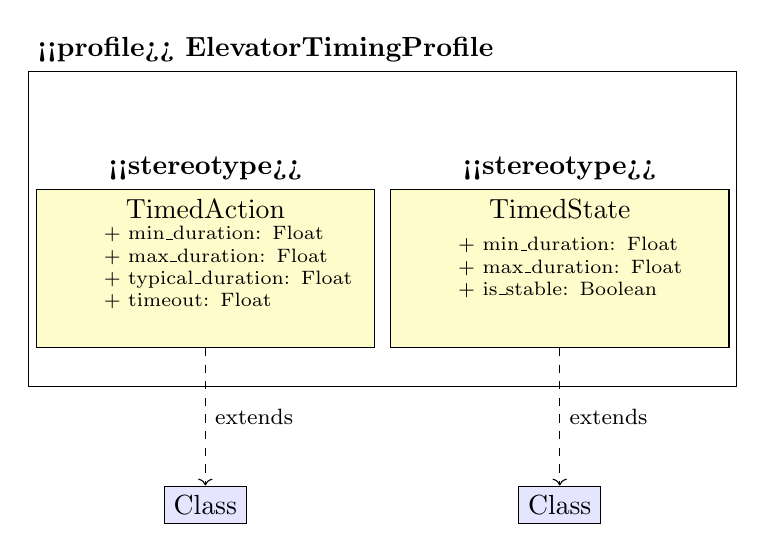
\begin{tikzpicture}
		\node[draw, rectangle, minimum width=9cm, minimum height=4cm] (profile) at (0,0) {};
		\node[above right] at (profile.north west) {\textbf{<<profile>> ElevatorTimingProfile}};
		
		\node[draw, rectangle, fill=yellow!20, minimum width=4.3cm, minimum height=2cm] (timed) at (-2.25, -0.5) {};
		\node[above] at (timed.north) {\textbf{<<stereotype>>}};
		\node[below] at (timed.north) {TimedAction};
		\node[text width=3cm, font=\scriptsize] at (timed.center) {
			\begin{tabular}{l}
				+ min\_duration: Float \\
				+ max\_duration: Float \\
				+ typical\_duration: Float \\
				+ timeout: Float \\
			\end{tabular}
		};
		
		\node[draw, rectangle, fill=yellow!20, minimum width=4.3cm, minimum height=2cm] (state) at (2.25, -0.5) {};
		\node[above] at (state.north) {\textbf{<<stereotype>>}};
		\node[below] at (state.north) {TimedState};
		\node[text width=3cm, font=\scriptsize] at (state.center) {
			\begin{tabular}{l}
				+ min\_duration: Float \\
				+ max\_duration: Float \\
				+ is\_stable: Boolean \\
			\end{tabular}
		};
		
		\node[draw, rectangle, fill=blue!10] (class) at (-2.25, -3.5) {Class};
		\draw[->, dashed] (timed) -- (class) node[midway, right, font=\footnotesize] {extends};
		
		\node[draw, rectangle, fill=blue!10] (class2) at (2.25, -3.5) {Class};
		\draw[->, dashed] (state) -- (class2) node[midway, right, font=\footnotesize] {extends};
	\end{tikzpicture}
\end{document}